%%====================%%
%%  Part III Project  %%
%%====================%%

\documentclass[aps,prd,reprint,preprintnumbers,showpacs,floatfix,nofootinbib,superscript address]{revtex4-2}
\usepackage[utf8]{inputenc}
\usepackage{parskip}
\usepackage{amssymb}
\usepackage{stix}
\usepackage{hhline}
\usepackage{amsmath}
\usepackage{mathtools}
\usepackage[dvipsnames]{xcolor}
\usepackage{xspace}
\usepackage{multirow,tabularx}
\usepackage{siunitx}
\usepackage{multirow}
\usepackage{graphicx}
\usepackage{xstring}
\usepackage{etoolbox}
\usepackage{notoccite}
\usepackage{natbib}
\usepackage{mathrsfs}
\usepackage{lineno}
\usepackage{tensor}
\usepackage{stackengine,scalerel}
\usepackage{accents}
\usepackage{tikz}
\usepackage{listings}
\allowdisplaybreaks
\parskip 1mm
\parindent 2mm

%%===========================%%
%%  Part III Project Macros  %%
%%===========================%%

%	The Planck mass
\newrobustcmd{\Planck}{%
	{M_{\text{Pl}}}%
}

%	The Riemannian covariant derivative
\newrobustcmd{\rD}[1]{%
	\tensor{\mathring{\nabla}}{#1}%
}

%	The Riemann-Cartan covariant derivative
\newrobustcmd{\rcD}[1]{%
	\tensor{\nabla}{#1}%
}

%	The Riemann tensor
\newrobustcmd{\rR}[1]{%
	\tensor{\mathring{R}}{#1}%
}

%	The Riemann-Cartan tensor
\newrobustcmd{\rcR}[1]{%
	\tensor{R}{#1}%
}

%	Irreducible parts of the torsion
\newrobustcmd{\T}[2][placeholder]{%
	\IfEqCase{#1}{%
	{placeholder}{\tensor{T}{#2}}%
	{1}{\tensor[^{(1)}]{T}{#2}}%
	{2}{\tensor[^{(2)}]{T}{#2}}%
	{3}{\tensor[^{(3)}]{T}{#2}}%
	}%
	[\packageError{cosmicclass}{Symbol #1 is not an irreducible part!}{}]%
}

%	Irreducible parts of the multiplier
\newrobustcmd{\TLambda}[2][placeholder]{%
	\IfEqCase{#1}{%
	{placeholder}{\tensor{\lambda}{#2}}%
	{1}{\tensor[^{(1)}]{\lambda}{#2}}%
	{2}{\tensor[^{(2)}]{\lambda}{#2}}%
	{3}{\tensor[^{(3)}]{\lambda}{#2}}%
	}%
	[\packageError{cosmicclass}{Symbol #1 is not an irreducible part!}{}]%
}
 %some personal macros

\usepackage{hyperref}
\hypersetup{%
     colorlinks = true,%
     linkcolor = Blue,%
     citecolor = Blue,%
     filecolor = Blue,%
     urlcolor = Blue% 
     }%
\usepackage[capitalize]{cleveref} %always load this last in preamble

\newcommand{\signature}[2][8em]{%
  \begin{tabular}[t]{ p{#1} p{#1} }
    \strut\raggedleft
    \raisebox{-.5ex}[0pt][0pt]{\bfseries #2} & \\
    \cline{2-2}
    & \centering\scriptsize\itshape (signature)
  \end{tabular}
}

\usepackage[style=nejm, 
citestyle=numeric-comp,
sorting=none]{biblatex}
\addbibresource{Bibliography.bib}


\nocite{*}

\begin{document}
\title{Constraints on inflation from scale-invariant gravity}

\author{Prabhoda CS}
\affiliation{Department of Physics, Cavendish Laboratory, University of Cambridge}

\begin{abstract}

\textbf{TO BE WRITTEN}
\textit{Italics sections to be edited... and more}
\end{abstract}

\maketitle
\section{INTRODUCTION}

\indent The simplest model of the Big Bang theory naturally follows from General Relativity applied to a general isotropic and homogeneous universe (Friedmann Equations) combined with Hubble's observations (Hubble's Law). This theory describes a universe with a constant expansion rate. It is a highly successful theory, able to offer a comprehensive explanation for a lot of experimental observations such as the CMB, the abundance of light elements, large-scale structure and mainly, Hubble's Law. However, this theory has some fine-tuning problems as to be described in the next section \ref{The need for Inflation}. 

The inflationary theory was developed in a series of papers by Guth \cite{GuthOriginalPaper}, Linde \cite{LINDE1982389}, and Steinhardt \cite{PhysRevLett.48.1220} and is a paradigm that aims to explain the observed level of homogeneity and isotropy in the universe today. It posits that in the early universe, a small patch underwent a period of rapid exponential expansion where in all the initial inhomogeneities were wiped out. The main idea of the theory is as follows: during the early universe, there existed a homogeneous, isotropic field pervading through spacetime such that its potential energy was greater than its kinetic energy. This supplied the negative pressure required in the Einstein Field Equations (EFE) for gravity to become repulsive and cause the rapid exponential expansion required for inflation, with inflation ending once the kinetic term is of the order of the potential energy.

Being a paradigm, however, the inflationary model provides no fundamental principle from which one can predict the form and structure of the Inflaton field or its Lagrangian. It is phenomenological, providing constraints on the behavior of potential and different terms, but not giving them a particular form.

This paper aims to argue that a particularly satisfying and immensely rich inflationary model can be arrived at by arguing for our Inflaton lagrangian, in the presence of gravity, to be locally scale invariant. 

Scale invariance in cosmology seems quite an attractive hypothesis given the nearly scale-invariant spectrum of primordial fluctuations as measured by Planck and WMAP. We also see that during inflation, the approximately deSitter metric $\text{d}s^2 = \frac{1}{H\eta}(\text{d}\eta^2 - \text{d}\Vec{x}^2)$ remains unchanged for a scale change corresponding to $\Vec{x} \rightarrow \lambda \Vec{x} \,\, \text{and} \,\, \eta \rightarrow \lambda \eta$ (where $\text{d}\eta =  \frac{\text{d}t'}{a(t')}$ is the conformal time), it therefore stands to reason that any EFT defined on this background must be scale invariant too, perhaps even locally. Much of the Starobinsky potential's success also arises from including the $R^2$ term in the Lagrangian, given $[R^2] = 4$ in natural units, its coefficient is naturally dimensionless and therefore invariant under change of scale $g_{\mu\nu} \rightarrow \Omega^2 g_{\mu\nu}$, for $\Omega$ constant. Appendix \ref{Appendix B} contains the mapping from the theory developed here to Starobinsky, showing we can arrive at that particular potential from gauged scale invariance. 

Another approach to inflationary cosmology is to consider metric-affine theories. This is done through the inclusion of the Holst invariant, a quantity that is already scale-invariant, in the Lagrangian. This has been explored in \cite{Salvio_2022} and \cite{pradisi2022equivalence}. The potential achieved in \cite{Salvio_2022} is identical to the one obtained through demanding scale invariance in \cite{barker2024poincaregaugetheoryconformal}, and the translation between the variables in the two theories will be given in Appendix \ref{Appendix A}. Finally, when considering the classical action of the Standard Model, dropping the Higgs mass terms, one finds that it too is scale-invariant and can be extended to be conformally invariant \cite{bars2014local}.

These investigations may hint towards a fundamental principle out of which these arise as limits - \textit{the inflaton potential arising} due to the gauging of this scale invariance, i.e., conformal symmetry.

This paper is structured as follows: Section \ref{The need for Inflation} explains some of the problems with the naive big bang model. Section \ref{Inflation} explains how the introduction of a scalar field that violates the strong energy condition helps us resolve these issues and derives the formulae and tools necessary to analyse the particular model that we will present in section \ref{Scale Invariant Gravity}. This section will take up most of the content of the paper and will analyse the various regimes and scenarios that the model accommodates. Finally, section \ref{Section 5??} 5?? will compare the model with observational data.


\section{The need for Inflation}\label{The need for Inflation}
\subsection{Horizon Problem}
In this section, we will show that given the standard assumed expansion rate in the Big Bang model, we cannot satisfactorily explain the near-perfect uniformity of the CMB. This is because, given the rate of expansion, there is no way for distant regions of the CMB to have once been causally connected.
Given the Friedmann Equations and defining the Hubble constant $H = \frac{\dot{a}}{a}$,
\begin{equation} \label{1}
    \dot{\rho} = -3(\rho + p)H
\end{equation}
\begin{equation} \label{2}
    \Ddot{a} = -\frac{4\pi G}{3} (\rho + 3p)a
\end{equation}
\begin{equation}    \label{3}
    H^2 + \frac{k}{a^2} = \frac{8 \pi G}{3} \rho
\end{equation}
From the continuity equation \ref{1}, we have:
\begin{equation} \label{4}
    \frac{\mathrm{d}  \ln(\rho)}{\mathrm{d} \ln(a)} = -3(1+w)
\end{equation}
Where, $w = \frac{p}{\rho}$. We can solve this equation to get $\rho \propto a^{-3(1+w)}$. In combination with Friedmann equation \ref{3} for a flat universe $k = 0$, we get the scale factor $a$ as a function of time $a(t)$.
\begin{equation}    \label{5}
    a(t) = \begin{cases}
        t^{2/3(1+w)} & w \neq -1 \\
        e^{Ht} & w = -1
    \end{cases}
\end{equation}
Now, we can define the comoving horizon ($\tau$) as the causal horizon or the maximum distance a light ray can travel between times 0 and $t$.
\begin{equation}    \label{6}
    \tau \equiv \int_{0}^{t} \frac{\mathrm{d} t'}{a(t')} = \int_{0}^{a} \frac{\mathrm{d}a}{H a^2} = \int_{0}^{a} \mathrm{d} \ln(a) \frac{1}{aH}
\end{equation}
Therefore, for a conventional Big Bang model, the causal horizon $\tau$ for a universe with $w \geq 0$ increases with time. In plain words, this means that the fraction of the universe with each other increases with time.
\begin{equation}
    \tau \propto a^{1/2(1+3w)} \implies \tau = \begin{cases}
        a & \text{Radiation Dominated} \\
        a^{1/2} & \text{Matter Dominated}
    \end{cases}
\end{equation}
The comoving horizon increasing with time implies that comoving scales (comoving scale is not the same as the physical scale) entering the cosmic horizon now were not in causal contact during the CMB decoupling! However, the anisotropy of the CMB is about one part in $10^{-5}$, posing a problem to the conventional big bang model to explain how these distant regions of the CMB managed to regulate their temperatures to such an accurate degree.

\subsection{Flatness Problem}
Despite the presence of mass and energy in our universe, the large-scale structure of our spacetime is approximately Euclidean (flat). To see whether this is a stable equilibrium, we return to Friedmann equation \ref{3} and defining $\rho_{\text{crit}} = 3H^2(a)$ and $\Omega(a) = \frac{\rho(a)}{\rho_{\text{crit}}}$, we get
\begin{equation}
    1 - \Omega(a) = \frac{-k}{(aH)^2}
\end{equation}
Differentiating this equation and using the Friedmann equations, we get,
\begin{equation}
    \frac{\mathrm{d}\Omega}{\mathrm{d} \ln a} = (1+3w)\Omega(\Omega-1)
\end{equation}
Looking at this, we can see that $\Omega = 1  \implies \rho = \rho_{crit}$ is an unstable equilibrium and slight perturbations can make the universe not flat, i.e., $k \neq 0$. This means that in the standard big bang model, matter density has to be extremely fine-tuned to fit the requirement $\rho = \rho_{crit}$, which seems unlikely.

The theory of inflation attempts to resolve the need for extreme fine-tuning of the initial conditions of the universe by positing a period of exponential expansion. The next section shows how this theory solves the two problems stated above.

\section{Inflation}\label{Inflation}
Looking at both the problems highlighted in the previous section, we see that the comoving Hubble radius ($(aH)^{-1}$) plays an important role
\begin{equation}    \label{10}
    \tau = \int_{0}^{a} \mathrm{d} \ln (a) \frac{1}{aH}
\end{equation}
\begin{equation} \label{11}
    1 - \Omega (a) = \frac{-k}{(aH)^2}
\end{equation}
If the comoving Hubble radius was decreasing, this means that large scales entering the present universe were inside the horizon before inflation. By equation \ref{11}, it also means that $\rho = \rho_{crit}$ is a stable equilibrium as the solution $\Omega = 1$ is an attractor during inflation.

A decreasing comoving horizon directly implies a period of accelerated expansion as seen by taking it's derivative
\begin{equation}
    \frac{\mathrm{d}}{\mathrm{d}t} \frac{1}{aH} <  0 \implies \frac{-\Ddot{a}}{(aH)^2} < 0 \implies \ddot{a} > 0
\end{equation}
Given that $\ddot{a} > 0$ and Friedmann equation \ref{2}, we see that $\frac{\rho}{3} < p \implies w < - \frac{1}{3}$. This is a violation of the strong energy condition.

So far, we have described the physical implications of inflation and it's effects. In the following section, we shall describe the physical conditions under which such an exponential expansion can arise. 

\subsection{Non-Canonical Scalar Field Inflation} \label{Non-Canonical Scalar Field Inflation}
The simplest models of inflation involve a scalar field $\phi$ (The Inflaton Field) that acts as the perfect fluid with $w < -\frac{1}{3}$ such that upon coupling with gravity through the Einstein-Hilbert action, it can provide the repulsive force in the Friedmann equations for the accelerated expansion.

In this section, we shall work with a general non-canonical scalar field and derive the equations of motion and relevant parameters for such a scalar field. This will provide us with the necessary groundwork for what is to come later in our model.
\begin{equation}\label{12}
    S = \int \mathrm{d}^4 x \sqrt{-g} \left[ g^{\mu \nu} \frac{K(\phi)}{2} \partial_{\mu}\phi \partial_{\nu} \phi  - V(\phi) \right]\
\end{equation}
Since during the inflationary period, we assume a de Sitter space (minus the perturbations), the FLRW metric is given by $g_{\mu \nu}= \text{diag}[1,-a^2(t),-a^2(t),-a^2(t)]$ making $\sqrt{-g} = a^3(t)$. We also assume that the scalar field is homogeneous and, therefore only varies with time, allowing us to drop the gradient term. The action then becomes: 
\begin{equation} \label{13}
    S = \int \text{dt}\text{d}^3\text{x} \; \text{a}^3(t) \left[ \frac{K(\varphi)}{2}\dot{\varphi}^2 - V(\varphi) \right]
\end{equation}
We vary the action and upon integrating by parts we get,
\begin{equation}
    \delta S = - \int \text{dt}\,\text{d}^3\textbf{x} \; \left[ a^3 K \ddot{\varphi} + a^3K_{,\varphi} \frac{\dot{\varphi}^2}{2}  +  3\dot{a} a^2 K \dot{\varphi} + a^3V_{,\varphi}  \right]\delta \varphi
\end{equation}
Setting this variation to zero, we get the equation of motion for a non-canonical scalar field.
\begin{equation} \label{16}
    K \ddot{\varphi} + \dot{\varphi} \left(\frac{K_{,\varphi} \dot{\varphi}}{2} + 3H K \right) + V_{,\varphi}   = 0
\end{equation}
We see this aligns with the canonical scalar field when we set $K = 1$, getting  $ \ddot{\varphi} +  3H \dot{\varphi}  + V_{,\varphi}   = 0$. While this equation is nice, it turns out to be more useful in cosmology to record how the inflaton field changes with respect to the e-folding time ($N = \int H \text{d}t$). For this, let us take an aside and given the action \ref{12}, derive the energy-momentum tensor.
\begin{equation}
    T_{\mu\nu} = \frac{2}{\sqrt{-g}} \frac{\delta S}{\delta  g^{\mu \nu}} = \frac{\partial \mathcal{L}}{\partial (\partial^\mu \phi)} \partial_\nu \phi - g_{\mu\nu} \mathcal{L}
\end{equation}
Using this, and simplifying the final expression we get, the energy density and the pressure of the fluid are as follows: 
\begin{align}
    \rho &= \frac{K(\varphi)}{2} \dot{\varphi}^2 + V(\varphi) \nonumber \\
    p &= \frac{K(\varphi)}{2} \dot{\varphi}^2 - V(\varphi)
\end{align}
Using the third Friedmann equation \ref{3}, we get:
\begin{equation}    \label{Friedmann Eqn 2}
    3 M_p^2H^2 = \frac{K(\varphi)}{2} \dot{\varphi}^2 + V(\varphi)
\end{equation}
Upon differentiating this expression with respect to time and using \ref{16}, we get:
\begin{equation}
    2 M_p^2 \dot{H} = -  K \dot{\varphi}^2
\end{equation}
Now that we have all the relevant parameters as functions of the field, we can look at equation \ref{16} and replace the time derivative there with the derivative with respect to the e-folding time N. Using $\text{d}N = H \text{d}t$, we get our final answer of the field evolution as a differential equation with respect to N.
\begin{widetext}
\begin{subequations}
\begin{align}\label{21}
    K\frac{\text{d}^2\varphi}{\text{d}N^2} +3 K \frac{\text{d}\varphi}{\text{d}N}  - \frac{K^2}{2M_p^2} \left(\frac{\text{d}\varphi}{\text{d}N} \right)^3  +  \frac{K_{,\varphi}}{2}  \left(\frac{\text{d}\varphi}{\text{d}N} \right)^2 +  \left( 3 M_p^2 - \frac{K}{2} \left(\frac{\text{d}\varphi}{\text{d}N} \right)^2 \right) \frac{\text{d}\ln \text{V}(\varphi)}{\text{d} \varphi} = 0    
\end{align}
\end{subequations}
\end{widetext}
\subsection{Slow Roll Inflation}
The acceleration equation for universe dominated by the inflaton field with the energy density $\rho_{\phi}$ and pressure $p_{\phi}$ is given by Friedmann equation \ref{2},
\begin{equation}
    \frac{\ddot{a}}{a} = -\frac{4\pi G}{3} (\rho +3p) = -\frac{8\pi G}{3} ({\dot{\phi}}^2 - V(\phi)) 
\end{equation}
We see that if we can get $\ddot{a} > 0$ by requiring $\dot{\phi}^2 << |V(\phi)|$. This period is called slow roll because when this condition is satisfied, it corresponds to the scalar field slowly rolling down its potential hill. The accelerated expansion will also only be satisfied for a long period if we require $|\ddot{\phi}| << 3H\dot{\phi} \sim |V,_{\phi}|$. 

We can rewrite these two slow-roll conditions with the two slow-roll parameters $\epsilon$ and $\eta$ and requiring that $\epsilon_V << 1$ and $\eta_V << 1$ during the slow roll. 
\begin{equation}
    \epsilon_V = \frac{1}{2K}  \left( \frac{V,_{\phi}}{V} \right)^2 \,\,\,\,\,\,\,\,\ \eta_V = \left| \frac{V,_{\phi\phi}}{V} \right|
\end{equation}
We can also write down the Hubble Slow Roll parameters (HSR), which are easily computable for our case of a non-canonical action:
\begin{align}
    \epsilon_H &= -  \left( \frac{\dot{H}}{H^2} \right) = \frac{K(\phi)}{2 M_p^2} \left( \frac{\text{d}\phi}{\text{d}N} \right)^2  \nonumber \\
    \eta_H &= \epsilon_H - \frac{1}{2 \epsilon_H} \left( \frac{\text{d}\epsilon_H}{\text{d}N} \right)
\end{align}
Inflation ends exactly when the HSR hits one, that is, $\epsilon_H = 1$.

So far, these arguments only provide restrictions on the potential of the scalar field $\phi$ but make no attempt to motivate the form of the potential or the action principle for the field from first principles. Thus, we see that the theory of inflation refers to a whole host of theories that aim to explain the mechanism behind the period of exponential expansion that occurred when the universe was around $\geq 10^{-34}s$ old.

\textit{One of the ways to arrive at the action principle of the inflaton field is to take a leaf out of the playbook of many successful QFTs and to hypothesize a gauge condition. This is the approach that shall be taken in this project and explained more in the next section.}


\section{Scale Invariant Gravity} \label{Scale Invariant Gravity}
Having laid the groundwork, we now come to the primary study of this project. This is based on the paper \cite{barker2024poincaregaugetheoryconformal} mainly and will follow up on the idea and analyze the theory with the inclusion of gravity. This immediately makes the theory much richer, producing various inflationary scenarios such as hilltop, plateau (Starobinsky-like), and even power law/ exponential potentials.

The theory of General Relativity is one of mankind's most rigorous scientific theories, is self-consistent and so far, all tests of GR have been shown to be in agreement with the theory. However, we do not \textit{a priori} know that the theory of general relativity can be extended to arbitrary energy (/length) scales. It is widely accepted that at high enough energy scales, those comparable to the Planck scale, GR breaks down. 

An interesting possibility to consider is that GR as we know it, with the Einstein-Hilbert Lagrangian being proportional to the Ricci Scalar, is a low-energy extrapolation of a more fundamental scale-invariant theory that describes physics at higher energies. 

In the argument that follows, we derive the most general conformally invariant action with non-irrelevant couplings of the inflaton field and gravity. We do not consider terms proportional to the curvature squared, even though this is a perfectly legal and general extension of the model. It is easy to show that this results in a two-field inflation model. We find, however, that the following model, which we will derive, is quite general and accounts for a lot of behaviors seen in the potentials derived through other means. Let us begin by exploring this possibility with a spin-0 scalar field model that reduces to the Klein-Gordon equation at the lowest order of perturbation.
\begin{equation} \label{25}
    S = \int \mathrm{d}^4 x \sqrt{-g} \frac{1}{2} \left[ \partial_\mu \delta \varphi \partial^\mu \delta \varphi - m^2   \delta\varphi^2   \right] + \text{gravity}
\end{equation}
Under local rescalings, the metric and the scalar transform as $g_{\mu\nu} \rightarrow e^{2\rho} g_{\mu\nu} $ and  $\varphi \rightarrow e^{-\rho}\varphi$ respectively. To ensure the kinetic terms retain their form, we introduce the Weyl vector $B_\mu$ which transforms as such $B_{\mu} \rightarrow B_\mu - \partial_\mu \rho$ under the gauge transformation (going back to the roots of the word) and define the covariant derivative $D_\mu = \partial_\mu - B_\mu$. To remove the explicit mass scale $m$ appearing in the Lagrangian \ref{25}, we add a compensator scalar field $\phi \rightarrow e^{-\rho}\phi$. For the gravity sector of the Lagrangian, let us see how the Christoffel symbol transforms under a local rescaling:
\begin{equation}
    \Gamma^{\alpha}_{\beta \gamma} \rightarrow \Gamma^{\alpha}_{\beta \gamma} +(\delta^{\alpha}_{\beta} \partial_\gamma \rho + \delta^{\alpha}_{\gamma} \partial_{\beta} \rho - g_{\beta \gamma}g^{\alpha \tau}\partial_{\tau}\rho)
\end{equation}
Defining a new connection that is conformally covariant using $B_\mu$ and using that to define the new curvature scalar, we get the Weyl curvature scalar:
\begin{align}
    \mathring{\Gamma}^{\alpha}_{\beta \gamma} &= \Gamma^{\alpha}_{\beta \gamma} + (\delta^{\alpha}_{\beta} B_{\gamma} + \delta^{\alpha}_{\gamma} B_{\beta} - g_{\beta \gamma}g^{\alpha \tau}B_{\tau}) \nonumber \\
    \mathcal{R} &= R - 6 B_{\mu} B^{\mu} - 6 \nabla_\mu B^\mu
\end{align}
Putting all this together, we get the most general conformally invariant action (assuming linearity in the curvature)
\begin{widetext}
\begin{subequations} \label{28a}
\begin{align}
    S =\int \text{d}^4\text{x} \; \sqrt{-g} &\; \left[ ( \beta \varphi^2 + \gamma \phi \varphi +\alpha \phi^2) R - 6( \beta \varphi^2 + \gamma \phi \varphi +\alpha \phi^2) (B_{\mu} B^{\mu} + \nabla_\mu B^\mu) \right. \nonumber \\
    &\quad \left. +\frac{\epsilon}{2} D_{\mu}\varphi D^{\mu}\varphi + \frac{\sigma}{2} D_{\mu}\varphi D^{\mu}\phi + \frac{\nu}{2} D_{\mu}\phi D^{\mu}\phi \right. \left. - \frac{\mu^2}{2} \phi^2 \varphi^2 + \frac{\lambda}{2} \varphi^4 + \frac{\kappa}{2} \phi^4 - \frac{\xi}{16} H_{\mu\nu}H^{\mu\nu} \right]  
\end{align}
\end{subequations}
\end{widetext}
A point to note here is the abundance of dimensionless parameters. We can remove any two by rescaling our fields, but we will leave it in this form until necessary. In the proceeding discussions, we shall set $\lambda = \kappa = 0$, this can be reinstated in the end, once the dynamics have been analyzed and the final inflaton potential is revealed.

In the equation above, we find two scalar fields. This makes analyzing the equations of motion harder. However, we have a redundant degree of freedom granted to us through the Weyl invariance we demanded the action possess. Looking at the units of $[\phi] = 2$, which is inverse length. Since the action is written down to be invariant under any choice of scale, we can choose a particular local length scale such that the field $\phi$ no longer appears dynamical, that is, rescale the metric and fields such that $\phi(\text{x}^\mu) = \phi_0$. The reparametrizations that allow us to do this are :
\[
g_{\mu \nu}\rightarrow\frac{\phi_0}{\phi}\,g_{\mu \nu},\quad 
\varphi\rightarrow\frac{\phi}{\phi_0}\,\varphi,\quad 
B_{\mu}\rightarrow B_{\mu} - \partial_{\mu}\ln(\phi)\,.
\] 
The resulting action in the Jordan Frame therefore reads:
\begin{equation}\label{29}
\begin{aligned}
\mathcal{L} &= \Bigl(\beta\, \varphi^2 + \gamma\, \phi_0\, \varphi + \alpha\, \phi_0^2\Bigr)
\Bigl(R - 6\, B_{\mu} B^{\mu} - 6\, \nabla_{\mu} B^\mu\Bigr) \\
&\quad + \frac{\epsilon}{2} \Bigl(\partial_{\mu}\varphi - \Bigl(\varphi + \frac{\sigma}{\epsilon}\,\phi_0\Bigr)B_{\mu}\Bigr)
\Bigl(\partial^{\mu}\varphi - \varphi\,B^{\mu}\Bigr) \\
&\quad - \frac{\mu^2}{2}\, \phi_0^2\,\varphi^2 
+ \frac{\nu\,\phi_0^2}{2}\,B_{\mu} B^{\mu} 
- \frac{\xi}{16}\,H_{\mu\nu} H^{\mu\nu}\,.
\end{aligned}
\end{equation}
In accordance with \cite{barker2024poincaregaugetheoryconformal}, we can send $\nu \rightarrow \infty$, to give us a Proca field $B_\mu$, (which could be a dark matter candidate \cite{Lasenby_2016}). In this regime, we can neglect the kinetic term corresponding to the Proca field, and it can be eliminated using the equations of motion as
\begin{equation}\label{30}
B_\mu = \frac{1}{2}\,\partial_\mu \ln\Bigl((\epsilon-12\beta)\,\varphi^2 + (\sigma-12\gamma)\,\phi_0\,\varphi + (\nu-12\alpha)\,\phi_0^2\Bigr)\,.
\end{equation}
and \ref{29} becomes:
\begin{widetext}
\begin{subequations}\label{33a}
\begin{align}
S = \int d^4x\, \sqrt{-g} \Biggl[ (\alpha\, \phi_0^2 + \beta\, \varphi^2 + \gamma\, \phi_0\,\varphi)R - 12\beta \Biggl\{1 - \frac{\phi_0^2}{48\beta\, V}\Bigl[(\sigma-12\gamma)^2 - 4(\epsilon-12\beta)(\nu-12\alpha)\Bigr]\Biggr\}
(\partial_{\mu}\varphi\, \partial^{\mu}\varphi) - \frac{\mu^2}{2}\,\phi_0^2\,\varphi^2 \Biggr],
\end{align}
\end{subequations}
\end{widetext}
where $V = [(\epsilon - 12\beta) \varphi^2 + (\sigma - 12\gamma) \phi_0 \varphi + (\nu - 12\alpha)\phi^2_0]$. Now, by means of the following conformal transformation 
\[
g_{\mu\nu}\rightarrow \Omega^2\,g_{\mu\nu},\quad\text{with}\quad \Omega^2 = \frac{M_p^2}{2(\alpha\,\phi_0^2+\beta\,\varphi^2+\gamma\,\phi_0\,\varphi)},
\]
we can move from the Jordan frame to the Einstein frame and separate the Einstein-Hilbert action and the inflaton action. Denoting $M_p/\sqrt{2} = M$, we get:
\begin{widetext}
\begin{subequations}\label{33a}
\begin{align}
S = \int d^4x\, \sqrt{-g} &\Biggl[ M^2\, R - \,\frac{M^2}{(\alpha\,\phi_0^2+\beta\,\varphi^2+\gamma\,\phi_0\,\varphi)}
\frac{24\beta}{2}\Biggl\{1 - \frac{\phi_0^2}{48\beta\,V}\Bigl[(\sigma-12\gamma)^2-4(\epsilon-12\beta)(\nu-12\alpha)\Bigr]\Biggr\} \nonumber\\[2mm]
&\quad - \frac{3M^2}{2}\,\frac{(2\beta\,\varphi+\gamma\,\phi_0)^2}{(\alpha\,\phi_0^2+\beta\,\varphi^2+\gamma\,\phi_0\,\varphi)^2}\,(\partial_{\mu}\varphi\,\partial^{\mu}\varphi) - \frac{M^4}{(\alpha\,\phi_0^2+\beta\,\varphi^2+\gamma\,\phi_0\,\varphi)^2}\,\frac{\mu^2}{2}\,\phi_0^2\,\varphi^2 \Biggr].
\end{align}
\end{subequations}
\end{widetext}
Denoting $A(\varphi) = (\beta\varphi^2+\gamma\phi_0\varphi+\alpha\phi_0^2)$ and $V(\varphi) = (\epsilon - 12\beta) \varphi^2 + (\sigma - 12\gamma) \phi_0  \varphi + (\nu - 12\alpha)\phi^2_0$. There are 6 free parameters here $\{ \beta, \gamma, \alpha , \epsilon, \sigma, \nu \}$. Using the redundancy in our choice of parameters in \ref{28a}, we can reparametrize the fields $\varphi$ and $\phi_0$ and the parameters to absorb two of these dimensionless parameters. Therefore, we can choose
\[
\begin{split}
\text{V} &= \left[(\epsilon - 12\beta)\,\varphi^2 + (\sigma - 12\gamma)\,\phi_0\,\varphi + (\nu - 12\alpha)\,\phi_0^2\right] \\
         &= k\,*\left[\beta\,\varphi^2 + \gamma\,\phi_0\,\varphi + \alpha\,\phi_0^2\right]
\end{split}
\]
Now only 4 dimensionless parameters still remain free; $\{k, \beta, \gamma, \alpha \}$.
\begin{equation}
    \begin{pmatrix}
        \epsilon \\ \sigma \\ \nu 
    \end{pmatrix}
    = (12+k)
    \begin{pmatrix}
        \beta \\ \gamma \\ \alpha
    \end{pmatrix}
\end{equation}
Discriminant $D = (\sigma -12 \gamma )^2-4 (\nu -12 \alpha ) (\epsilon -12 \beta ) = k^2 (\gamma^2 - 4\alpha \beta) = (\frac{k}{12+k})^2 (\sigma^2 -4 \epsilon \nu)$. This simplifies the equation \ref{33a} and we can write it as:
\begin{widetext}
    \begin{equation} 
    \begin{aligned}
        S &= \int \text{d}^4\text{x} \sqrt{-g} [ M^2 R + \frac{M^2}{2} \left[-\frac{36 \beta}{A} + \frac{\phi_0^2 (\gamma^2 - 4\beta\alpha)(k-6)}{2 A^2}\right] (\partial_\mu \varphi \partial^\mu \varphi) -  \frac{M^4}{A^2} \frac{\mu^2}{2} \phi^2_0 \varphi^2 ] 
    \end{aligned}
\end{equation}
\end{widetext}
where again, $A =\beta\,\varphi^2 + \gamma\,\phi_0\,\varphi + \alpha\,\phi_0^2$ and $M_p/\sqrt{2} = M$ has been used in the equation above.

The action is finally of the form $S = S_{\text{EH}} + S_{\text{INFLATON}}$. The inflaton action has the form of a non-canonical scalar field, with the kinetic and potential coefficients, $K(\varphi)$ and $V(\varphi)$.

\subsection{Solution and Different Regimes}
We now have all the relevant pieces to analyse the model, given the information in section \ref{Non-Canonical Scalar Field Inflation}. For the starting Lagrangian \ref{28a}, we have developed a variable dictionary given the parameter and field definition redundancy as:
\begin{equation} \label{35}
    \begin{pmatrix}
        \epsilon \\ \sigma \\ \nu 
    \end{pmatrix}
    = (12+k)
    \begin{pmatrix}
        \beta \\ \gamma \\ \alpha
    \end{pmatrix}
\end{equation}
Given these parameters, we were able to simplify the Lagrangian \ref{28a} to one of the form $S_{EH} + S_{INFLATON}$. Now, looking at only the inflaton potential, we have: 
\begin{equation}
    S_{INFLATON} = \int \text{d}^4x \left[ \frac{K(\varphi)}{2} \partial_\mu \varphi \partial^\mu \varphi - V(\varphi)\right]
\end{equation}
where, the kinetic and potential terms, $K(\varphi)$ and $V(\varphi)$ are given by:
\begin{align}
    \text{K}(\varphi) &= \left[-\frac{36 \beta M^2}{(\beta \varphi^2 + \gamma\phi_0\varphi + \alpha \phi_0^2)} + \frac{M^2 \phi_0^2 (\gamma^2 - 4\beta\alpha)(k-6)}{2 (\beta \varphi^2 + \gamma\phi_0\varphi + \alpha \phi_0^2)^2}\right] \label{37} \\
    \text{V}(\varphi) &= \frac{ M^4 \mu^2 \phi^2_0 \varphi^2}{2(\beta \varphi^2 + \gamma\phi_0\varphi + \alpha \phi_0^2)^2} \label{38}
\end{align}
To canonicalize the action, that is, to write it in the form with no kinetic coefficient:
\begin{equation}
    S_{\text{INFLATON}} = \int \text{d}^4x \sqrt{-g} \left[ \frac{1}{2}\partial_\mu \tilde{\varphi}\partial^\mu \tilde{\varphi} - V(\varphi(\tilde{\varphi})) \right]
\end{equation}
we will need to redefine the field such that:
\begin{equation} \label{40}
    \tilde{\varphi}(\varphi) = \int_0^{\varphi} \sqrt{K(x)} \text{d}x
\end{equation}
However, for the $K(\varphi)$ derived in this model \ref{37}, there exists no closed-form analytical solution to the integral \ref{40}. While we present the results of numerical integration of the above kinetic term in the next section, here, we will look at various regimes to understand the behaviour of this model in different limits. 

\subsubsection{\textbf{CASE I }: $k \gg 1$}

Assuming $\beta \ll \phi_0^2(\gamma^2 - 4\alpha\beta)(k-6)$, we get the field redefinition ($\gamma^2 > 4\alpha\beta$):
\begin{equation}
    \frac{d\tilde{\varphi}}{d\varphi} = \left[ \sqrt{\frac{k}{2}} \frac{M \phi_0 D}{\beta \varphi^2  +\gamma \phi_0 \varphi +\alpha \phi^2_0} \right]
\end{equation}
This gives:
\begin{equation}
    \varphi(\tilde{\varphi}) = \frac{\phi_0}{2\beta} \left[\gamma - \sqrt{\gamma^2 - 4\alpha \beta} \tanh\left(\frac{\tilde{\varphi}}{M_p\sqrt{k}}-c \right) \right]
\end{equation}
Using this in the potential, we get:
\begin{equation}
    V(\tilde{\varphi}) =  2\mu^2 \cosh^2(X)  \left [ \frac{f(X) }{2\gamma^2 - D^2 + 2\gamma f(2X)} \right]^2
\end{equation}
Where,  $f(X) = \gamma \cosh(X)  + D \sinh(X)$. $X = \left(\frac{\tilde{\varphi}}{M_p\sqrt{k}} - c\right)$ and $D = \sqrt{\gamma^2 - 4\alpha\beta}$
Plotting this potential, we get figure \ref{CASE I potential} 
\begin{figure}[h!]
    \centering
    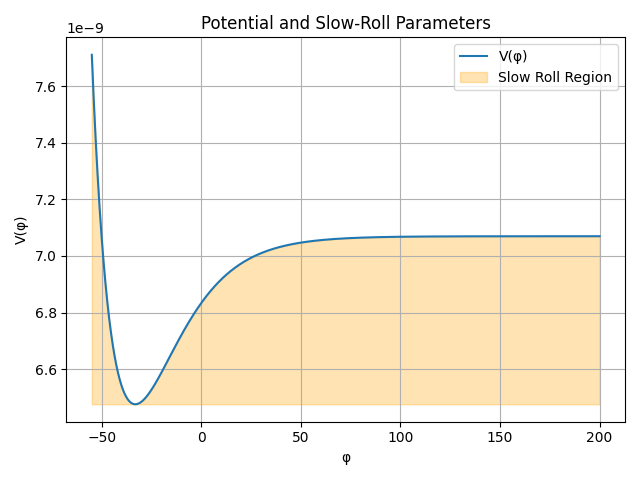
\includegraphics[width=0.4\textwidth]{Python/Figures/New Potenial with gravity.png}
    \caption{CASE I}
    \label{CASE I potential}
\end{figure}
Here the parameter choices made in \ref{CASE I potential} are: $\mu = 1 ,M_p = 20\sqrt{2} ,\phi_0 = 3.\gamma = 20 ,\alpha = -50,\beta = 1, K = 1, c = -2$, where $K = \sqrt{\frac{k}{2}}$

\subsubsection{\textbf{CASE II}: $k = 6$}
Assuming $k=6$,  we get the field redefinition:
\begin{equation}
    \frac{d\tilde{\varphi}}{d\varphi} = \sqrt{\left[\frac{-36 \beta M^2}{(\beta \varphi^2 + \gamma\phi_0\varphi + \alpha \phi_0^2)} \right]}
\end{equation}
For the field redefinition to make sense, we require $\gamma^2 < 4\alpha \beta$, this gives us:
\begin{equation}
    \tilde{\varphi} = \frac{\phi_0}{2\beta} \left[\gamma + \sqrt{4\alpha\beta - \gamma^2} \sinh\left(\frac{\varphi}{3\sqrt{2}M_p}\right) \right]
\end{equation}
The resulting potential is:
\begin{equation}
    V(\tilde{\varphi}) = \frac{\mu^2}{2} \frac{1}{(4\alpha\beta-\gamma^2)^2} \text{sech}^4\left(\frac{\tilde{\varphi}}{3\sqrt{2}M_p} \right) \left[\frac{\gamma }{2} + \sqrt{\alpha\beta-\frac{\gamma^2}{4}} \sinh\left(\frac{\tilde{\varphi}}{3\sqrt{2}M_p} \right) \right]^2
\end{equation}
This shows the same behavior as \cite{barker2024poincaregaugetheoryconformal} for small values of $\varphi$; it is an asymptotically exponentially damped version of the same graph.

\subsubsection{\textbf{NUMERICAL ANALYSIS}}
Stitching together the two regimes, we can see that $K(\varphi)$ interpolates between the two regimes based on values of $\varphi \, \, \text{and}\, \,k$. For intermediate $k$, both terms contribute, leading to a non-trivial kinetic structure, which is not always integrable.

For $\varphi \rightarrow 0$, the $\frac{1}{A^2(\varphi)}$ term dominates, giving a hyperbolic tangent contribution, a power-law structure/steep potential close to zero. For $\varphi \rightarrow \infty$, the $\frac{1}{A(\varphi)}$ term dominates,  giving a hyperbolic sine contribution, providing an exponentially damped solution leading to a plateau-like shape. 

Finally, using Python, we can numerically integrate equation \ref{40}, interpolate the function $\tilde{\varphi}(\varphi)$, invert it, and use it to attain the shape of the true potential \ref{38}. The parameters below have been chosen such that the scalar spectral index $n_s = 1 + \frac{1}{K}(2\eta_V - 6 \epsilon_V -\sqrt{2\epsilon_V}\lambda_K)$, \cite{chung2003running} ($\lambda_K = M_p \frac{K_{,\varphi}}{K}$) is close to the experimental value of 0.968 at around 60 efolds.

\begin{figure}[h!]
    \centering
    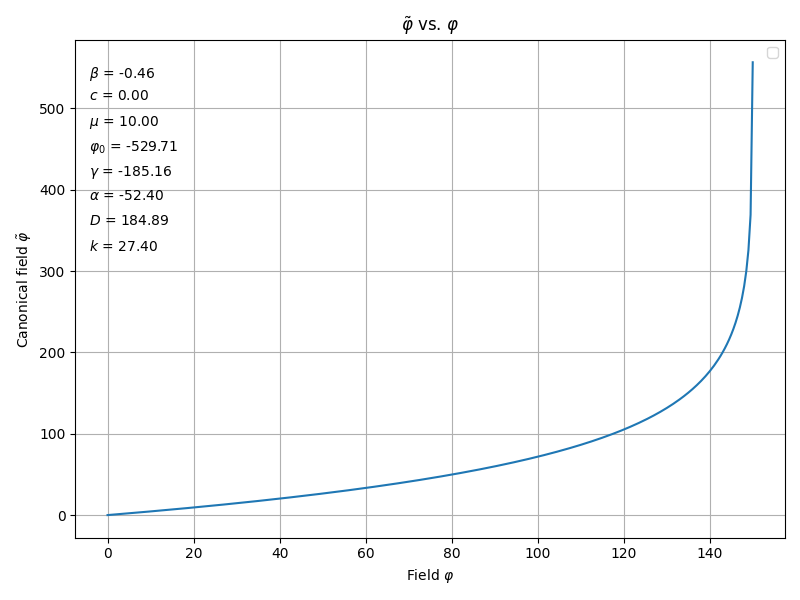
\includegraphics[width=0.7\textwidth]{Python/Figures/Redefinition with correct parameters.png}
    \caption{$\tilde{\varphi}$ vs $\varphi$}
    \label{Canonical field vs field}
\end{figure}
For this redefinition, we get the potential as such:

\begin{figure}[h!]
    \centering
    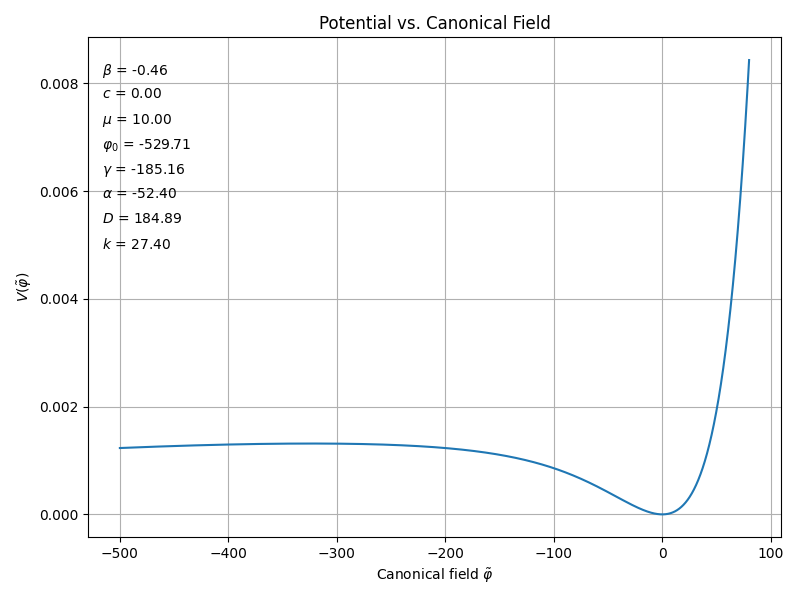
\includegraphics[width=0.7\textwidth]{Python/Figures/Potential with correct parameters.png}
    \caption{V(\varphi) vs \varphi}
    \label{Full Potential}
\end{figure}

The slow roll variables, $\epsilon_V \, \, \text{and} \, \, \eta_V$ also reach one around zero as shown in the below graph.

\begin{figure}[h!]
    \centering
    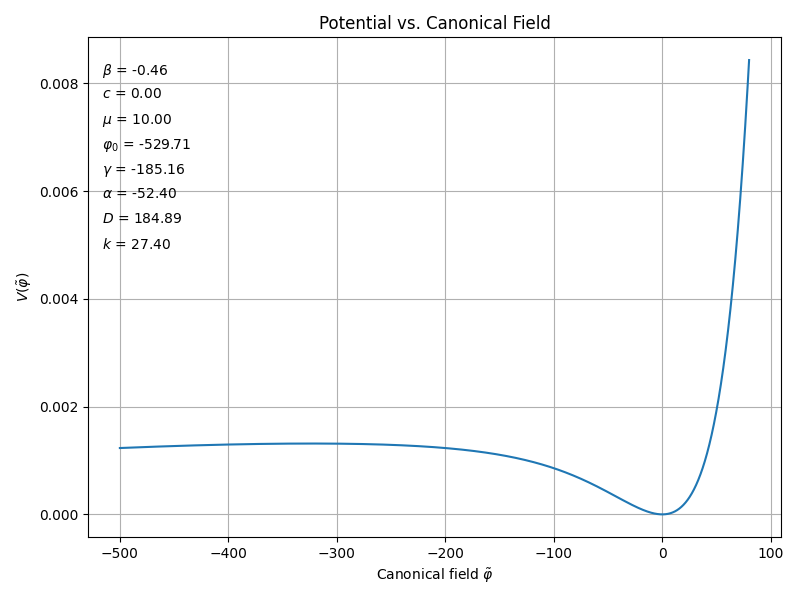
\includegraphics[width=0.7\textwidth]{Python/Figures/Potential with correct parameters.png}
    \caption{V(\varphi) vs \varphi}
    \label{Full Potential}
\end{figure}


\newpage
$\,$
\newpage

\appendix

\section{Translating variables from Salvio to Barker} \label{Appendix A}

In the paper \cite{Salvio_2022}, the authors derived an inflaton potential using metric affine gravity. The motivation here is to give inflation a geometrical explanation. 
By starting with this action, 
\begin{equation}
    S = \int \text{d}^4\text{x} \sqrt{-g} (\alpha \mathcal{R} + \beta \mathcal{R}' + c \mathcal{R}'^{2})
\end{equation}
Where $\mathcal{R}'$ is the Holst Invariant, a \textit{scale-invariant} quantity. The potential derived finally is: 
\begin{equation}
    U(\omega) = \frac{1}{4 c'} \left[ \frac{M_{p}^{2}}{4} \text{sinh}(\text{X}(\omega)) - \beta  \right]^2
\end{equation}
where
\begin{equation}
    \text{X}(\omega) = \sqrt{\frac{2}{3}} \frac{\omega}{M_{p}} + \text{tanh}^{-1} \left(\frac{4 \beta}{\sqrt{M_{p}^{4}+16 \beta^2}} \right)
\end{equation}

Barker \cite{barker2024poincaregaugetheoryconformal} derives a similar form of the potential starting with a scale-invariant scalar field. The resulting potential there is:

\begin{equation}
    U'(\varphi) = \frac{\mu^2 \phi_{0}^{4}}{2} \left[ \frac{\sigma}{2} + \sqrt{\nu - \frac{\sigma^2}{4}} \text{sinh}\left( \text{X}'(\varphi) \right)  \right]^2
\end{equation}
where
\begin{equation}
    \text{X}'(\varphi) =  \frac{\varphi}{\phi_0 \sqrt{\nu - \frac{\sigma^2}{4}}} - \frac{c}{\phi_0 \sqrt{\nu - \frac{\sigma^2}{4}}}
\end{equation}

The substitutions necessary to transform back and forth from these models are: 

\begin{align}
    \phi_0 &= g \sqrt{\frac{3}{2}} M_p  \nonumber \\
    \mu &= g^{-1} \frac{1}{6 \sqrt{2 c'}}  \nonumber \\
    \sigma &= - g^{-1} \frac{8 \beta}{M_{p}^{2}}  \nonumber \\
    \nu &= g^{-2} \left( 1 + \frac{16 \beta^2}{M_{p}^{4}} \right) \nonumber \\
    c  &= -\sqrt{\frac{3}{2}} M_{p} \text{tanh}^{-1} \left(\frac{4 \beta}{\sqrt{M_{p}^{4}+16 \beta^2}} \right)
\end{align}

where $g$ is a dimensionless coupling constant, this tells us that the Barker model has an extra degree of freedom that we can absorb into the definitions of the other variables.

\section{Reduction to the Starobinsky Model} \label{Appendix B}

The Starobinsky Model Lagrangian includes a quadratic curvature (a scale invariant) term in the Einstein-Hilbert action. When the curvature is high, the quadratic term dominates and drives inflation away from an unstable de Sitter fixed point \cite{Cecchini_2024}. Looking at a particular sector in our theory from Lagrangian \ref{28a} where we have chosen $\lambda = \beta$,
\begin{equation} \label{B1}
    S =\int \text{d}^4\text{x} \sqrt{-g} \left[ (\alpha \phi_0^2 + \beta \varphi^2)\mathcal{R} - \frac{\lambda}{2} \varphi^4 \right]  
\end{equation}
Upon utilization of the Euler-Lagrange equation on the $\varphi$ field $2 \beta \varphi R - 2\beta \varphi^3 = 0$, if $\varphi \neq 0$, the other solution $\varphi^2 = R$, gives us \ref{B2}. This can be re-written as:
\begin{equation} \label{B2}
    S =\int \text{d}^4\text{x} \sqrt{-g} \left[ \alpha \phi_0^2 \mathcal{R} + \frac{\beta}{2} \mathcal{R}^2  \right]
\end{equation}
 We can see that this action, a particular regime of the general lagrangian \ref{28a}, is equivalent to the Starobinsky model. Therefore, to match this with our model, we use our variable dictionary \ref{35}

To reduce to the above equations to \ref{B2}, we choose: $\gamma = 0, k = -12$, and $\beta$ negative, giving $\epsilon = \sigma = \nu = 0$. Our $K(\varphi)$ and $V(\varphi)$ given in \ref{37} and \ref{38} therefore reduce to:
\begin{align}
    \text{K}(\varphi) &= \left[\frac{36 M^2 \beta^2 \varphi^2}{ (\beta \varphi^2 + \alpha \phi_0^2)^2}\right] \\
    \text{V}(\varphi) &= \frac{ M^4 \lambda \varphi^4}{2(\beta \varphi^2 + \alpha \phi_0^2)^2}    
\end{align}
Giving the field redefinition:
\begin{align}
    \tilde{\varphi}(\varphi) &= 3M \ln\left(1 + \frac{\beta \varphi^2}{\alpha \phi_0^2} \right) \nonumber \\
    \varphi^2(\tilde{\varphi}) &=  \frac{\alpha}{\beta} \phi_0^2\left [ \exp\left(\frac{\tilde{\varphi}}{3M}\right) -1\right]
\end{align}
Using this in the potential, we get the Starobinsky-like potential:
\begin{equation}
    \text{V}(\tilde{\varphi}) = \frac{ M_p^4}{8 \beta}  \left(1 - \exp\left(-\frac{\sqrt{2} \tilde{\varphi}}{3 M_p}\right)\right)^2
\end{equation}
In comparison with the Starobinsky Model, \cite{ivanov2022analytic}, \cite{lust2024starobinsky}, we see that the parameters $m^2 \approx \frac{3}{4} 10^{-10}M_p^2 =\frac{M_p^2}{8\beta}$, giving us $\beta \approx 10^{9}$. We also note that the terms $\alpha, \phi_0$ drop out of the final potential, giving us the Starobinsky behaviour of a one-parameter potential. \textit{The only caveat for this potential is the appearance of the $\frac{1}{3}$ factor in the exponential compared to the $\frac{1}{\sqrt{3}}$ factor in \cite{lust2024starobinsky}, is due to their choice to use the first power of the scalar field to couple to the Ricci scalar, compared to our second powers}.

\section{Reduction to Barker Model}
For the Lagrangian \ref{28a} to reduce to Barker, we require $\beta = \gamma =0$; this can be done through the choice $k \rightarrow\infty$. To ensure that the conformal transformation we did on the way is not singular, we require $\alpha$. Converting the parameters from $\alpha, \beta, \gamma$ to $\epsilon, \sigma, \nu$ in the $K,V$ formulae:

We get:
\begin{align}
    \text{K}(\varphi) &= \left[\frac{M^2 \phi_0^2 (\sigma^2 - 4\epsilon\nu)k}{2 (\epsilon \varphi^2 + \sigma\phi_0\varphi + \nu \phi_0^2)^2}\right] \label{C4}  \\
    \text{V}(\varphi) &= \frac{ k^2 M^4 \mu^2 \phi^2_0 \varphi^2}{2(\epsilon \varphi^2 + \sigma\phi_0\varphi + \nu \phi_0^2)^2}
\end{align}
In the limit $k \rightarrow\infty$, the field redefinition becomes:
\begin{equation}
    \varphi(\tilde{\varphi}) = \frac{\phi_0}{2\epsilon} \left[\sigma - \sqrt{\sigma^2 - 4\epsilon \nu} \tanh\left(\frac{\tilde{\varphi}}{M_p\sqrt{k}}-c \right) \right]
\end{equation}
The field $\varphi$ is bounded by:
\begin{equation}
    \frac{\phi_0}{2\epsilon} \left[\sigma - \sqrt{\sigma^2 - 4\epsilon \nu}\right] < \varphi < \frac{\phi_0}{2\epsilon} \left[\sigma + \sqrt{\sigma^2 - 4\epsilon \nu}  \right]
\end{equation}

\newpage

\printbibliography
\end{document}